\documentclass[a4paper,12pt]{book}
\usepackage[utf8]{inputenc}
\usepackage{graphicx}
\usepackage{titlesec}
\usepackage{hyperref}

\titleformat
{\chapter} % command
[display] % shape
{\bfseries\Huge\itshape} % format
{\small{Tic-Tac-Toe Machine Learning Workshop}} % label
{0.5ex} % sep
{
	\rule{\textwidth}{1pt}
	\vspace{1ex}
	\centering
} % before-code
[
\vspace{-0.5ex}%
\rule{\textwidth}{0.3pt}
] % after-code





% Default fixed font does not support bold face
\DeclareFixedFont{\ttb}{T1}{txtt}{bx}{n}{12} % for bold
\DeclareFixedFont{\ttm}{T1}{txtt}{m}{n}{12}  % for normal

% Custom colors
\usepackage{color}
\definecolor{deepblue}{rgb}{0,0,0.5}
\definecolor{deepred}{rgb}{0.6,0,0}
\definecolor{deepgreen}{rgb}{0,0.5,0}

\usepackage{listings}

% Python style for highlighting
\newcommand\pythonstyle{\lstset{
		language=Python,
		basicstyle=\ttm,
		otherkeywords={self},             % Add keywords here
		keywordstyle=\ttb\color{deepblue},
		emph={MyClass,__init__},          % Custom highlighting
		emphstyle=\ttb\color{deepred},    % Custom highlighting style
		stringstyle=\color{deepgreen},
		frame=tb,                         % Any extra options here
		showstringspaces=false            % 
}}


% Python environment
\lstnewenvironment{python}[1][]
{
	\pythonstyle
	\lstset{#1}
}
{}

% Python for external files
\newcommand\pythonexternal[2][]{{
		\pythonstyle
		\lstinputlisting[#1]{#2}}}

% Python for inline
\newcommand\pythoninline[1]{{\pythonstyle\lstinline!#1!}}

\begin{document}
	
	\author{Martin Mrugała\\Patryk Walczak\\Filip Szymczak\\Bartek Żyła\\Maciej Zalewski}
	\title{\Huge{\bf{Machine Learning Project\\Tic-Tac-Toe}}}
	\date{\emph{16th June, 2020}}
	
	\frontmatter
	\maketitle

	\tableofcontents
	
	\mainmatter
	\chapter{Introduction}
	\section{Standard Tic-tac-toe}
	According to the definition in the Oxford Dictionary of English, Tic-tac-toe is a game in which two players seek to complete a row of either three noughts or three crosses drawn alternately in the spaces of a grid of nine squares.
		\begin{figure}[!h]
		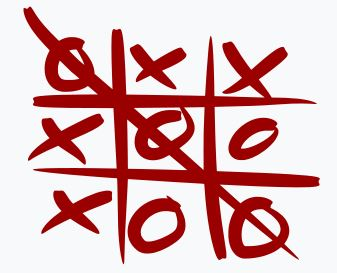
\includegraphics{./Images/1.jpg}
		\centering
		\caption{A completed game of Tic-tac-toe\protect\footnotemark.}
		\label{fig:Capture1}
	\end{figure}
	\footnotetext{Source of the image: \url{https://en.wikipedia.org/wiki/Tic-tac-toe}}
	And as it turns out, there are 255 168 possible games. So this means that, with the help of the reinforcement learning, a bot may be trained to mastery. 
	\newpage
	\section{Our implementation}
	
	\begin{python}
		class MyClass(Yourclass):
		def __init__(self, my, yours):
		bla = '5 1 2 3 4'
		print bla
	\end{python}

	
	\backmatter
	% bibliography, glossary and index would go here.
	
\end{document}